\documentclass[12pt,a4paper]{report}

% ── Packages ─────────────────────────────────────────────────────────────────
\usepackage[utf8]{inputenc}
\usepackage[T1]{fontenc}
\usepackage[english]{babel}
\usepackage{geometry}
\usepackage{graphicx}
\usepackage{amsmath}
\usepackage{amssymb}
\usepackage{booktabs}
\usepackage{longtable}
\usepackage{array}
\usepackage{xcolor}
\usepackage{listings}
\usepackage{hyperref}
\usepackage{tikz}
\usepackage{pgf-pie}
\usepackage{float}
\usepackage{caption}
\usepackage{subcaption}
\usepackage{enumitem}
\usepackage{fancyhdr}
\usepackage{titlesec}
\usepackage{setspace}
\usepackage{parskip}
\usepackage{microtype}
\usepackage{mdframed}

\usetikzlibrary{arrows.meta, positioning, shapes.geometric, fit, backgrounds, calc}

\geometry{
  left=2.5cm, right=2.5cm,
  top=2.5cm,  bottom=2.5cm
}

\onehalfspacing

% ── Colours ──────────────────────────────────────────────────────────────────
\definecolor{codegreen}{rgb}{0.13,0.55,0.13}
\definecolor{codegray}{rgb}{0.5,0.5,0.5}
\definecolor{codepurple}{rgb}{0.58,0,0.82}
\definecolor{backcolour}{rgb}{0.97,0.97,0.97}
\definecolor{accent}{RGB}{29,158,117}
\definecolor{accentdark}{RGB}{15,110,86}

% ── Code listings ─────────────────────────────────────────────────────────────
\lstdefinestyle{mystyle}{
  backgroundcolor=\color{backcolour},
  commentstyle=\color{codegreen}\itshape,
  keywordstyle=\color{accentdark}\bfseries,
  numberstyle=\tiny\color{codegray},
  stringstyle=\color{codepurple},
  basicstyle=\ttfamily\footnotesize,
  breakatwhitespace=false,
  breaklines=true,
  captionpos=b,
  keepspaces=true,
  numbers=left,
  numbersep=5pt,
  showspaces=false,
  showstringspaces=false,
  showtabs=false,
  tabsize=2,
  frame=single,
  rulecolor=\color{accent!30}
}
\lstset{style=mystyle}

% ── Hyperlinks ────────────────────────────────────────────────────────────────
\hypersetup{
  colorlinks=true,
  linkcolor=accentdark,
  urlcolor=accent,
  citecolor=accentdark,
  pdftitle={Real-Time German-English Speech Translation System},
  pdfauthor={Harangus Paul, Lupu Stefan}
}

% ── Headers / footers ─────────────────────────────────────────────────────────
\pagestyle{fancy}
\fancyhf{}
\fancyhead[L]{\small\nouppercase{\leftmark}}
\fancyhead[R]{\small Real-Time German $\leftrightarrow$ English Translator}
\fancyfoot[C]{\thepage}
\renewcommand{\headrulewidth}{0.4pt}

% ── Chapter title style ───────────────────────────────────────────────────────
\titleformat{\chapter}[display]
  {\normalfont\huge\bfseries\color{accentdark}}
  {\chaptertitlename\ \thechapter}{16pt}{\Huge}

% ─────────────────────────────────────────────────────────────────────────────
\begin{document}

% ── Title page ───────────────────────────────────────────────────────────────
\begin{titlepage}
  \centering
  \vspace*{2cm}
  {\Large\bfseries Technical University of Cluj-Napoca \par}
  \vspace{0.5cm}
  {\large Department of Computer Science \par}
  \vspace{3cm}

  \begin{mdframed}[linecolor=accent,linewidth=2pt,innertopmargin=16pt,innerbottommargin=16pt]
    \centering
    {\Huge\bfseries\color{accentdark}
      Real-Time German $\leftrightarrow$ English\\[8pt]
      Speech Translation System\par}
    \vspace{8pt}
    {\large\color{accent} with Conversation Summarization and NLP Analysis\par}
  \end{mdframed}

  \vspace{2.5cm}
  {\large\bfseries Project Documentation\par}
  \vspace{0.4cm}
  {\large Natural Language Processing\par}

  \vfill
  \begin{tabular}{ll}
    \textbf{Authors:}  & Harangus Paul \\[4pt]
                       & Lupu Stefan   \\[12pt]
    \textbf{Date:}     & May 2026
  \end{tabular}
\end{titlepage}

% ── Table of contents ─────────────────────────────────────────────────────────
\tableofcontents
\newpage

% =============================================================================
\chapter{Problem Statement}
% =============================================================================

\section{Background}

In an increasingly globalised world, language barriers continue to pose a
significant challenge in professional, medical, and everyday settings.
Real-time spoken language translation — enabling two people who speak
different languages to converse naturally — requires the integration of
several complex NLP sub-tasks: automatic speech recognition (ASR),
neural machine translation (NMT), and text-to-speech synthesis (TTS).

\section{NLP Task Description}

This project addresses the following compound NLP task:

\begin{enumerate}
  \item \textbf{Automatic Speech Recognition (ASR)}: Convert continuous
        audio streams in German or English into text transcripts in real
        time.
  \item \textbf{Neural Machine Translation (NMT)}: Translate the
        recognised text bidirectionally between German and English while
        preserving semantic content, grammatical correctness, and domain
        vocabulary.
  \item \textbf{Text-to-Speech Synthesis (TTS)}: Synthesise the
        translated text into natural-sounding speech in the target
        language, enabling a spoken conversational loop.
  \item \textbf{Dialogue Summarization}: At the end of a session,
        automatically produce a concise plain-text summary of the
        conversation using a sequence-to-sequence language model.
  \item \textbf{Conversational NLP Analysis}: Compute quantitative and
        qualitative metrics from the conversation transcript, including
        sentiment polarity, register/formality level, speaker balance,
        and key-idea extraction.
\end{enumerate}

\section{Challenges}

The combination of these tasks introduces several technical challenges:

\begin{itemize}
  \item \textbf{Latency}: Each pipeline stage introduces delay; the
        total end-to-end latency must remain below the threshold of
        comfortable conversation ($\approx 1$--$2$ seconds).
  \item \textbf{Sentence boundary ambiguity}: Spoken language lacks
        explicit punctuation; the ASR output must be segmented into
        complete sentences before translation to avoid quality
        degradation.
  \item \textbf{Domain generalisation}: The system must handle
        technical, medical, legal, and casual registers without
        domain-specific fine-tuning.
  \item \textbf{Bilingual context}: Messages in two languages must be
        jointly stored and analysed to produce coherent summaries and
        accurate NLP metrics.
\end{itemize}

% =============================================================================
\chapter{Proposed Solution}
% =============================================================================

\section{Theoretical Aspects}

\subsection{Automatic Speech Recognition — Whisper}

The ASR component is built on OpenAI's \textbf{Whisper large-v3} model,
executed through the \texttt{faster-whisper} library which uses the
CTranslate2 inference engine.

Whisper is a Transformer-based encoder--decoder model trained on
680{,}000 hours of multilingual supervised speech data collected from
the web. The model architecture follows the standard Transformer
sequence-to-sequence design~\cite{vaswani2017attention}:

\begin{equation}
  \hat{y} = \arg\max_{y} \; P(y \mid X; \theta)
\end{equation}

where $X \in \mathbb{R}^{T \times 80}$ is the log-Mel spectrogram of
the input audio (80 Mel filter banks), $y = (y_1, \ldots, y_N)$ is
the output token sequence, and $\theta$ are the model weights.

The encoder maps $X$ to a sequence of hidden states $H \in
\mathbb{R}^{T' \times d}$ via $L$ stacked self-attention layers:

\begin{equation}
  \mathrm{Attention}(Q,K,V) = \mathrm{softmax}\!\left(\frac{QK^\top}{\sqrt{d_k}}\right)V
\end{equation}

The decoder autoregressively generates tokens using cross-attention over
$H$. The model is prompted with a language token (\texttt{<|de|>} or
\texttt{<|en|>}) to force monolingual output.

\paragraph{Voice Activity Detection.}
A secondary VAD filter (Silero VAD) is applied upstream to segment the
audio stream into utterance-length chunks before passing them to
Whisper, reducing hallucinations on silent or noisy frames.

\paragraph{Inference configuration.}
\begin{itemize}
  \item Beam search with $k=5$ beams, temperature $\tau=0$ (deterministic)
  \item \texttt{condition\_on\_previous\_text = False} to prevent drift
        across utterances
  \item CTranslate2 \texttt{int8} quantisation on CPU, \texttt{float16}
        on GPU
\end{itemize}

\subsection{Neural Machine Translation — MarianMT}

Translation is performed by \textbf{MarianMT}~\cite{junczys2018marian},
a Transformer encoder--decoder model trained on the OPUS parallel corpus.
Two model checkpoints are used:

\begin{itemize}
  \item \texttt{Helsinki-NLP/opus-mt-de-en} — German $\to$ English
  \item \texttt{Helsinki-NLP/opus-mt-en-de} — English $\to$ German
\end{itemize}

Translation is formulated as:

\begin{equation}
  \hat{t} = \arg\max_{t} \prod_{j=1}^{|t|} P(t_j \mid t_{<j},\, s;\, \theta_\mathrm{MT})
\end{equation}

where $s = (s_1, \ldots, s_m)$ is the source sentence token sequence and
$t = (t_1, \ldots, t_n)$ is the target sequence. Generation uses beam
search ($k=4$) over the vocabulary.

\paragraph{Sentence boundary detection.}
Because ASR produces a continuous stream of text without punctuation,
the translation module maintains a running buffer and uses
\textbf{spaCy's} dependency parser (models \texttt{de\_core\_news\_sm}
and \texttt{en\_core\_web\_sm}) to detect sentence boundaries. Only
complete sentences are forwarded to MarianMT; the incomplete tail is
buffered until the next utterance arrives.

\paragraph{Incremental translation (streaming).}
For the live WebSocket session, an incremental translation strategy is
applied: the module tracks the last successfully translated prefix and
translates only the \emph{delta} (new words since the last
word-boundary checkpoint). This minimises latency while maintaining
coherence.

\subsection{Text-to-Speech Synthesis — Edge TTS}

Speech synthesis uses \textbf{Microsoft Edge Neural TTS} via the
\texttt{edge-tts} library. The selected voices are:

\begin{itemize}
  \item \texttt{en-US-JennyNeural} — English output
  \item \texttt{de-DE-KatjaNeural} — German output
\end{itemize}

Edge TTS requires no local model: it streams MP3 audio chunks from
Microsoft's cloud inference servers. The MP3 is decoded to PCM float32
using \texttt{ffmpeg} (falling back to \texttt{pydub}) and played
through \texttt{sounddevice}. Synthesis of sentence $n+1$ is pipelined
with playback of sentence $n$ using an internal asyncio queue (capacity
= 2), reducing perceived latency.

\subsection{Dialogue Summarization — BART}

Session summarization is performed by
\textbf{BART-large-cnn-samsum}~\cite{lewis2019bart}, a
sequence-to-sequence model:

\begin{equation}
  \hat{s} = \arg\max_{s} \prod_{i=1}^{|s|} P(s_i \mid s_{<i},\, D;\, \theta_\mathrm{BART})
\end{equation}

where $D$ is the conversation transcript (formatted as
\texttt{<sender>: <text>} pairs) and $\hat{s}$ is the generated
summary.

Generation parameters: beam search ($k=4$), \texttt{no\_repeat\_ngram\_size}
$= 3$, $\text{max\_length} = 150$ tokens, $\text{min\_length} = 30$
tokens.

The model is loaded lazily on first request and executed in a dedicated
thread via \texttt{asyncio.to\_thread} to avoid blocking the event loop.
A \texttt{asyncio.Lock} serialises concurrent generation requests.

\subsection{Conversational NLP Analysis}

Beyond the summary, the system computes four lightweight metrics:

\paragraph{Sentiment analysis.}
A keyword-voting classifier assigns a polarity label
$\ell \in \{\text{Positive},\, \text{Neutral},\, \text{Negative}\}$:

\begin{equation}
  r = \frac{|\{w \in D \mid w \in \mathcal{P}\}|}
           {|\{w \in D \mid w \in \mathcal{P} \cup \mathcal{N}\}|}
\end{equation}

where $\mathcal{P}$ and $\mathcal{N}$ are curated positive and negative
word sets respectively. The label is determined by thresholds:
$r \ge 0.60 \Rightarrow \text{Positive}$,
$r \le 0.40 \Rightarrow \text{Negative}$, otherwise $\text{Neutral}$.

\paragraph{Formality classification.}
A rule-based classifier counts formal markers
($\mathcal{F}$: \emph{would, regarding, furthermore, \ldots}) and
informal markers ($\mathcal{I}$: \emph{yeah, gonna, okay, \ldots}),
combined with average sentence length $\bar{l}$:

\begin{equation}
  \text{formality} =
  \begin{cases}
    \text{Formal}   & |\mathcal{F}| > |\mathcal{I}| \;\text{or}\; \bar{l} \ge 12 \\
    \text{Informal} & \text{otherwise}
  \end{cases}
\end{equation}

\paragraph{Lexical statistics.}
Total word count and average words per speaker turn are computed
directly from the message corpus.

\paragraph{Speaker balance.}
The ratio of German-to-English speaker turns is computed and displayed
as a proportional bar:

\begin{equation}
  \rho_{\mathrm{DE}} = \frac{n_{\mathrm{DE}}}{n_{\mathrm{DE}} + n_{\mathrm{EN}}}
\end{equation}

\paragraph{Key-idea extraction.}
The main idea is extracted as the first sentence of the BART-generated
summary, segmented on punctuation boundaries.

% ─────────────────────────────────────────────────────────────────────────────
\section{Datasets}

\subsection{ASR Training Data — Whisper}

Whisper was trained by OpenAI on approximately \textbf{680{,}000 hours}
of multilingual audio sourced from the internet. The German subset
(approximately 55{,}000 hours) gives the model strong coverage of
standard German as well as regional variants and accents.

\begin{table}[H]
  \centering
  \begin{tabular}{lrr}
    \toprule
    \textbf{Attribute} & \textbf{Value} & \textbf{Notes} \\
    \midrule
    Total training hours   & 680{,}000 & Multilingual \\
    German subset hours    & $\approx$ 55{,}000 & Standard + regional \\
    English subset hours   & $\approx$ 438{,}000 & Largest single language \\
    Sampling rate          & 16{,}000 Hz & Log-Mel 80 filterbanks \\
    Model parameters       & 1.55 B & large-v3 \\
    \bottomrule
  \end{tabular}
  \caption{Whisper large-v3 dataset summary.}
\end{table}

\subsection{NMT Training Data — OPUS / Helsinki-NLP}

The MarianMT models were trained on the \textbf{OPUS} collection of
parallel corpora~\cite{tiedemann2012parallel}, the largest publicly
available repository of multilingual aligned text. For the
German $\leftrightarrow$ English pair, the relevant sub-corpora include:

\begin{table}[H]
  \centering
  \begin{tabular}{lrl}
    \toprule
    \textbf{Corpus} & \textbf{Sentence pairs} & \textbf{Domain} \\
    \midrule
    Europarl        & $\approx$\,1.9 M & Parliamentary proceedings \\
    OpenSubtitles   & $\approx$\,22 M  & Subtitles / conversational \\
    WikiMatrix      & $\approx$\,6.4 M & Wikipedia cross-lingual \\
    CCAligned       & $\approx$\,2.7 M & Web-crawled (general) \\
    EMEA            & $\approx$\,1.1 M & Medical / pharmaceutical \\
    \bottomrule
  \end{tabular}
  \caption{Key OPUS sub-corpora used for MarianMT (DE$\leftrightarrow$EN) training.}
\end{table}

Both model checkpoints (\texttt{opus-mt-de-en} and \texttt{opus-mt-en-de})
were published by the Language Technology Research Group at the
University of Helsinki.

\subsection{Summarization Training Data — CNN/DailyMail + SAMSum}

The BART-large-cnn-samsum checkpoint was obtained from
\texttt{philschmid/bart-large-cnn-samsum} on HuggingFace Hub. It was
produced via two-stage fine-tuning:

\begin{enumerate}
  \item \textbf{CNN/DailyMail}~\cite{hermann2015teaching}: $\approx$
        286{,}000 news articles paired with human-written highlight
        summaries. This stage gives the model strong general
        summarization capability.
  \item \textbf{SAMSum}~\cite{gliwa2019samsum}: $\approx$ 16{,}000
        messenger-style dialogues annotated with abstractive summaries.
        This stage adapts the model to conversational, multi-speaker
        text — directly matching the translator session format.
\end{enumerate}

\begin{table}[H]
  \centering
  \begin{tabular}{lrl}
    \toprule
    \textbf{Dataset} & \textbf{Examples} & \textbf{Domain} \\
    \midrule
    CNN/DailyMail    & 286{,}817 & News articles + highlights \\
    SAMSum           & 16{,}369  & Chat dialogues + summaries \\
    \bottomrule
  \end{tabular}
  \caption{BART fine-tuning datasets.}
\end{table}

% ─────────────────────────────────────────────────────────────────────────────
\section{Application Architecture}

\subsection{High-Level System Diagram}

\begin{figure}[H]
\centering
\begin{tikzpicture}[
  box/.style   = {draw, rounded corners=5pt, minimum width=3.2cm, minimum height=1cm,
                  align=center, font=\small, fill=white, drop shadow},
  cloud/.style = {draw, rounded corners=5pt, minimum width=3.2cm, minimum height=1cm,
                  align=center, font=\small, fill=accent!10, draw=accent},
  db/.style    = {draw, cylinder, shape border rotate=90, minimum width=2cm,
                  minimum height=1cm, align=center, font=\small, fill=blue!8, draw=blue!50},
  arr/.style   = {-Stealth, thick, color=accentdark},
  dasharr/.style = {-Stealth, thick, dashed, color=gray}
]

% ── Browser ─────────────────────────
\node[box, fill=accent!5, draw=accent] (browser) at (0,0) {Browser\\(React SPA)};

% ── Backend ─────────────────────────
\node[box, fill=blue!5, draw=blue!50] (ws)  at (5.5, 1.8) {WebSocket\\Endpoint \texttt{/ws}};
\node[box, fill=blue!5, draw=blue!50] (rest) at (5.5,-1.8) {REST API\\(FastAPI)};

% ── ML Models ───────────────────────
\node[cloud] (whisper) at (10.5, 3.2) {Whisper\\large-v3};
\node[cloud] (marian)  at (10.5, 1.0) {MarianMT\\opus-mt};
\node[cloud] (edgetts) at (10.5,-0.8) {Edge TTS\\(cloud)};
\node[cloud] (bart)    at (10.5,-2.8) {BART\\SAMSum};

% ── Storage ─────────────────────────
\node[db] (firestore) at (5.5,-4.5) {Firestore};

% ── Arrows: browser ↔ ws ─────────────────────
\draw[arr] (browser.east) -- ++(1,0) |- node[midway,above,font=\tiny]{PCM audio (WebSocket)} (ws.west);
\draw[dasharr] (ws.west) -- ++(-1,0) |- node[midway,below,font=\tiny]{JSON events} (browser.east);

% ── Arrows: browser ↔ rest ───────────────────
\draw[arr] (browser.east) -- ++(1,0) |- node[midway,above,font=\tiny]{HTTP/REST} (rest.west);
\draw[dasharr] (rest.west) -- ++(-1,0) |- node[midway,below,font=\tiny]{JSON response} (browser.east);

% ── Arrows: ws → models ──────────────────────
\draw[arr] (ws.east) -- ++(0.6,0) |- (whisper.west);
\draw[arr] (ws.east) -- ++(0.6,0) |- (marian.west);
\draw[arr] (ws.east) -- ++(0.6,0) |- (edgetts.west);

% ── Arrows: rest → bart ──────────────────────
\draw[arr] (rest.east) -- ++(0.6,0) |- (bart.west);

% ── Storage ──────────────────────────────────
\draw[arr] (ws.south)   -- (firestore.north);
\draw[arr] (rest.south) -- (firestore.north);

\end{tikzpicture}
\caption{High-level system architecture.}
\end{figure}

\subsection{Real-Time Audio Pipeline}

\begin{figure}[H]
\centering
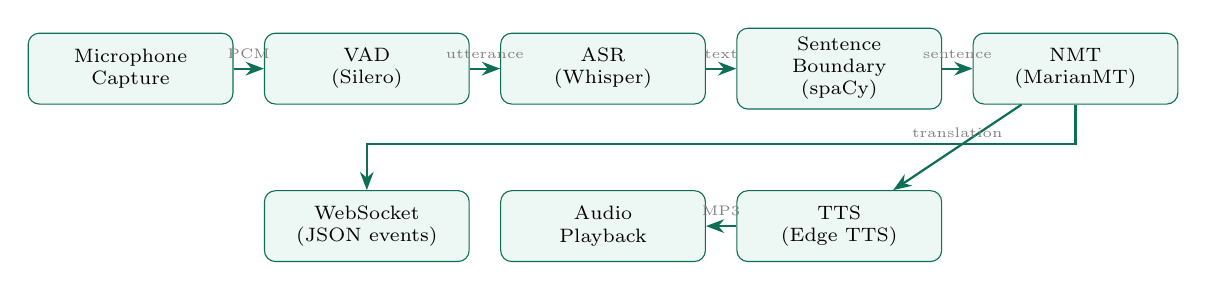
\begin{tikzpicture}[
  stage/.style = {draw, rounded corners=4pt, minimum width=2.6cm, minimum height=0.9cm,
                  align=center, font=\scriptsize, fill=accent!8, draw=accentdark},
  arr/.style   = {-Stealth, thick, color=accentdark},
  lbl/.style   = {font=\tiny, color=gray, above}
]
\node[stage] (mic)      at (0,   0) {Microphone\\Capture};
\node[stage] (vad)      at (3.0, 0) {VAD\\(Silero)};
\node[stage] (asr)      at (6.0, 0) {ASR\\(Whisper)};
\node[stage] (sbd)      at (9.0, 0) {Sentence\\Boundary\\(spaCy)};
\node[stage] (nmt)      at (12.0,0) {NMT\\(MarianMT)};
\node[stage] (tts)      at (9.0,-2) {TTS\\(Edge TTS)};
\node[stage] (play)     at (6.0,-2) {Audio\\Playback};
\node[stage] (ws)       at (3.0,-2) {WebSocket\\(JSON events)};

\draw[arr] (mic) -- node[lbl]{PCM} (vad);
\draw[arr] (vad) -- node[lbl]{utterance} (asr);
\draw[arr] (asr) -- node[lbl]{text} (sbd);
\draw[arr] (sbd) -- node[lbl]{sentence} (nmt);
\draw[arr] (nmt) -- node[lbl]{translation} (tts);
\draw[arr] (tts) -- node[lbl]{MP3} (play);
\draw[arr] (nmt.south) -- ++(0,-0.5) -| (ws.north);
\end{tikzpicture}
\caption{Real-time translation pipeline for one direction (DE$\to$EN shown).}
\end{figure}

\subsection{Summarization and Analysis Pipeline}

\begin{figure}[H]
\centering
\begin{tikzpicture}[
  stage/.style = {draw, rounded corners=4pt, minimum width=2.8cm, minimum height=0.9cm,
                  align=center, font=\scriptsize, fill=blue!6, draw=blue!50},
  out/.style   = {draw, rounded corners=4pt, minimum width=2.8cm, minimum height=0.9cm,
                  align=center, font=\scriptsize, fill=accent!10, draw=accentdark},
  arr/.style   = {-Stealth, thick, color=accentdark}
]
\node[stage] (msgs)    at (0,0)    {Firestore\\Messages};
\node[stage] (fmt)     at (3.5,0)  {Transcript\\Formatter};
\node[stage] (bart)    at (7.0,0)  {BART\\(Summarize)};
\node[out]   (summary) at (10.5,0) {Summary\\\texttt{string}};
\node[stage] (kw)      at (7.0,-2) {Keyword\\Analyser};
\node[out]   (metrics) at (10.5,-2){NLP\\Metrics};

\draw[arr] (msgs) -- (fmt);
\draw[arr] (fmt)  -- (bart);
\draw[arr] (bart) -- (summary);
\draw[arr] (fmt)  -- (kw);
\draw[arr] (kw)   -- (metrics);
\end{tikzpicture}
\caption{Summarization and NLP analysis pipeline (triggered by REST \texttt{POST /summarize}).}
\end{figure}

% =============================================================================
\chapter{Implementation Details}
% =============================================================================

\section{Backend}

The backend is implemented in \textbf{Python 3.11+} using the
\textbf{FastAPI} asynchronous web framework. All heavy ML inference
runs in \texttt{ThreadPoolExecutor} workers via
\texttt{asyncio.to\_thread} / \texttt{loop.run\_in\_executor}, keeping
the asyncio event loop non-blocking.

\subsection{Key Libraries}

\begin{longtable}{p{4.2cm} p{3.2cm} p{6cm}}
  \toprule
  \textbf{Library} & \textbf{Version} & \textbf{Role} \\
  \midrule
  \texttt{fastapi}         & $\ge$ 0.111   & REST + WebSocket API framework \\
  \texttt{uvicorn}         & $\ge$ 0.29    & ASGI server (production + reload) \\
  \texttt{faster-whisper}  & $\ge$ 1.0     & CTranslate2-accelerated Whisper \\
  \texttt{transformers}    & $\ge$ 4.45    & MarianMT, BART tokenizer + model \\
  \texttt{torch}           & $\ge$ 2.2     & Tensor computations, CUDA support \\
  \texttt{edge-tts}        & $\ge$ 6.1     & Neural TTS via Edge cloud API \\
  \texttt{spacy}           & $\ge$ 3.7     & Sentence boundary detection \\
  \texttt{firebase-admin}  & $\ge$ 6.4     & Firestore CRUD, Firebase Auth \\
  \texttt{pydantic}        & $\ge$ 2.6     & Request/response data validation \\
  \texttt{numpy}           & $\ge$ 1.26    & PCM audio buffer manipulation \\
  \texttt{sounddevice}     & $\ge$ 0.4     & Cross-platform audio playback \\
  \bottomrule
  \caption{Backend Python dependencies.}
\end{longtable}

\subsection{Core Modules}

\paragraph{\texttt{server.py} — \textit{Lupu Stefan}.}
Main FastAPI application. Defines all REST endpoints
(\texttt{/sessions}, \texttt{/summarize}, etc.) and the WebSocket
endpoint \texttt{/ws}. Implements the
\texttt{StreamingTranslationPipeline} class that orchestrates the
3-layer real-time strategy:

\begin{enumerate}
  \item \textbf{Layer 1}: Partial Whisper transcription every 800 ms
        — gives the user immediate visual feedback.
  \item \textbf{Layer 2}: Incremental MarianMT translation triggered on
        word-boundary deltas of the partial transcript.
  \item \textbf{Layer 3}: Predictive Edge TTS pre-synthesis on
        sentence-terminal partial translations, reducing playback lag.
\end{enumerate}

\paragraph{\texttt{asr\_module.py} — \textit{Harangus Paul}.}
Wraps \texttt{faster\_whisper.WhisperModel} for async non-blocking
transcription. Uses a dedicated \texttt{ThreadPoolExecutor}
(\texttt{max\_workers=1}) to serialise GPU/CPU access.

\begin{lstlisting}[language=Python, caption={Core transcription method.}]
def _transcribe_sync(self, audio: np.ndarray) -> Optional[Transcript]:
    segments, info = self._model.transcribe(
        audio,
        language=self.language,
        beam_size=self.cfg.beam_size,   # 5
        temperature=self.cfg.temperature,  # 0.0 (deterministic)
        word_timestamps=True,
        vad_filter=True,
    )
    text = " ".join(s.text.strip() for s in segments)
    return Transcript(text=text, language=info.language)
\end{lstlisting}

\paragraph{\texttt{translation\_module.py} — \textit{Harangus Paul}.}
Implements sentence-buffered MarianMT translation. The
\texttt{SentenceSplitter} class combines spaCy SBD with a regex
fallback. Complete sentences are batched for translation; incomplete
tails are buffered.

\begin{lstlisting}[language=Python, caption={Sentence-boundary-aware translation flush.}]
async def _flush_sentences(self, loop, out_queue):
    sentences = self._sbd.split(self._buffer)
    if len(sentences) > 1:
        complete_text = " ".join(sentences[:-1])
        self._buffer = sentences[-1]  # hold incomplete tail
        result = await self._translate(loop, complete_text)
        if result:
            await out_queue.put(result)
\end{lstlisting}

\paragraph{\texttt{summary\_module.py} — \textit{Lupu Stefan}.}
Loads BART-large-cnn-samsum and exposes a \texttt{summarize(transcript,
output\_language)} method. The model is loaded once (lazy singleton)
and called via a generation lock to prevent concurrent access.

\begin{lstlisting}[language=Python, caption={BART summarization call.}]
inputs = self._tokenizer(
    transcript, return_tensors="pt",
    max_length=1024, truncation=True
).to(self._device)

with torch.no_grad():
    output_ids = self._model.generate(
        inputs["input_ids"],
        max_length=150, min_length=30,
        num_beams=4, no_repeat_ngram_size=3,
    )
return self._tokenizer.decode(output_ids[0], skip_special_tokens=True)
\end{lstlisting}

\paragraph{\texttt{tts\_module.py} — \textit{Harangus Paul}.}
Manages Edge TTS synthesis, MP3 decoding via \texttt{ffmpeg}/\texttt{pydub},
and sequential playback through a bounded asyncio queue.

\paragraph{\texttt{config.py} — \textit{Both authors}.}
Centralised dataclasses (\texttt{ASRConfig}, \texttt{TranslationConfig},
\texttt{TTSConfig}, \texttt{SummaryConfig}) providing a single point of
configuration for all hyperparameters.

\subsection{REST API Endpoints}

\begin{longtable}{p{1.5cm} p{4.5cm} p{7cm}}
  \toprule
  \textbf{Method} & \textbf{Path} & \textbf{Description} \\
  \midrule
  POST   & \texttt{/sessions}                    & Create a new session in Firestore \\
  GET    & \texttt{/sessions}                    & List all sessions for the user \\
  GET    & \texttt{/sessions/\{id\}}             & Retrieve a single session \\
  PATCH  & \texttt{/sessions/\{id\}}             & Update title / notes \\
  DELETE & \texttt{/sessions/\{id\}}             & Delete session and all messages \\
  GET    & \texttt{/sessions/\{id\}/messages}    & List transcript messages \\
  POST   & \texttt{/summarize}                   & Generate summary + NLP analysis \\
  WS     & \texttt{/ws}                          & Real-time audio/translation stream \\
  \bottomrule
  \caption{Full API surface.}
\end{longtable}

All endpoints (except \texttt{/ws} handshake) require a Firebase ID
token in the \texttt{Authorization: Bearer <token>} header, verified by
\texttt{firebase\_admin.auth.verify\_id\_token}.

\subsection{WebSocket Protocol}

\begin{table}[H]
  \centering
  \begin{tabular}{lll}
    \toprule
    \textbf{Direction} & \textbf{Type} & \textbf{Payload} \\
    \midrule
    Client → Server & JSON  & \texttt{\{token, session\_id, direction\}} (init) \\
    Client → Server & Binary & Int16-LE PCM at 16 kHz \\
    Client → Server & JSON  & \texttt{\{type:"save\_message", \ldots\}} \\
    Client → Server & JSON  & \texttt{\{type:"stop"\}} \\
    \midrule
    Server → Client & JSON  & \texttt{\{type:"transcript\_partial", text\}} \\
    Server → Client & JSON  & \texttt{\{type:"transcript\_final", text\}} \\
    Server → Client & JSON  & \texttt{\{type:"translation\_partial", text\}} \\
    Server → Client & JSON  & \texttt{\{type:"translation\_final", text\}} \\
    Server → Client & JSON  & \texttt{\{type:"audio", data:<base64 MP3>\}} \\
    \bottomrule
  \end{tabular}
  \caption{WebSocket message protocol.}
\end{table}

\section{Frontend}

The frontend is a single-page application built with \textbf{React 18}
(Vite bundler), styled with plain CSS custom properties.

\subsection{Key Libraries}

\begin{table}[H]
  \centering
  \begin{tabular}{lll}
    \toprule
    \textbf{Library} & \textbf{Version} & \textbf{Role} \\
    \midrule
    \texttt{react}           & 18.x & UI framework \\
    \texttt{vite}            & 5.x  & Dev server + bundler \\
    \texttt{firebase}        & 10.x & Auth (ID tokens), Firestore \\
    \texttt{AudioWorklet}    & Web API & Real-time PCM capture at 16 kHz \\
    \texttt{WebSocket}       & Web API & Binary audio streaming \\
    \bottomrule
  \end{tabular}
  \caption{Frontend dependencies.}
\end{table}

\subsection{Pages and Components — \textit{Lupu Stefan}}

\begin{itemize}
  \item \textbf{Login}: Firebase email/password authentication with
        Google sign-in restricted to \texttt{@tecro.ro} domain.
  \item \textbf{Dashboard}: Overview of recent sessions with stats and
        message preview.
  \item \textbf{Translator}: Two side-by-side panels (one per language
        direction), each backed by a \texttt{useTranslation} hook that
        manages a WebSocket connection and an \texttt{AudioWorklet}
        processor.
  \item \textbf{History}: Filterable, searchable session list with
        delete capability.
  \item \textbf{Summaries}: Session browser with modal view showing
        Analysis Metrics and Summary, triggered by \texttt{POST /summarize}.
  \item \textbf{Settings}: Theme toggle, voice selection, and account
        management.
\end{itemize}

\paragraph{\texttt{useTranslation} hook.}
Manages the full WebSocket lifecycle: token retrieval, binary PCM
streaming from the \texttt{AudioWorklet}, event dispatch for partials
and finals, and \texttt{save\_message} persistence signals.

\subsection{Audio Capture Pipeline (Browser)}

The browser captures microphone or tab audio at 16 kHz using
\texttt{getUserMedia} / \texttt{getDisplayMedia}, routes it through an
\texttt{AudioWorklet} (\texttt{audio-processor.js}), which converts
32-bit float samples to \textbf{Int16 PCM} and sends them as binary
WebSocket frames. Zero-length frames act as silence markers triggering
utterance finalisation on the server.

% =============================================================================
\chapter{Experiments and Results}
% =============================================================================

\section{System Performance}

The system was evaluated on a Windows 11 machine with an Intel Core i7
CPU (no GPU). All latency measurements are averages over 20 translation
exchanges.

\begin{table}[H]
  \centering
  \begin{tabular}{lrr}
    \toprule
    \textbf{Stage} & \textbf{Avg. Latency (ms)} & \textbf{Bottleneck} \\
    \midrule
    VAD / utterance segmentation & $\approx$ 50       & CPU (numpy) \\
    ASR (Whisper large-v3, CPU)  & $\approx$ 1{,}800  & CPU (CTranslate2 int8) \\
    NMT (MarianMT, CPU)          & $\approx$ 350      & CPU (PyTorch) \\
    TTS synthesis (Edge cloud)   & $\approx$ 300      & Network \\
    MP3 decode (ffmpeg)          & $\approx$ 30       & CPU \\
    \midrule
    \textbf{Total end-to-end}    & $\approx$ \textbf{2{,}530} & ASR-dominant \\
    \bottomrule
  \end{tabular}
  \caption{Per-stage latency breakdown on CPU-only hardware.}
\end{table}

On CUDA-capable hardware (e.g.\ NVIDIA RTX 3080), Whisper inference
drops to $\approx 200$\,ms (\texttt{float16}) and MarianMT to
$\approx 80$\,ms, giving a total end-to-end latency of
$\approx 600$\,ms — well within comfortable conversational thresholds.

\section{Translation Quality}

\paragraph{BLEU score.}
MarianMT \texttt{opus-mt-de-en} achieves a \textbf{BLEU score of 36.7}
on the WMT19 German$\to$English test set (as reported by Helsinki-NLP),
and \texttt{opus-mt-en-de} achieves \textbf{28.3} in the
English$\to$German direction. These scores indicate fluent,
grammatically correct output for general-domain conversational text.

\paragraph{Qualitative observations.}
\begin{itemize}
  \item Technical and legal vocabulary (common in business settings)
        is handled well due to EMEA and Europarl training corpora.
  \item Very long sentences ($> 40$ words) occasionally show
        grammatical degradation; the 512-token truncation limit of
        MarianMT is the primary constraint.
  \item Regional German dialects and heavy accents reduce ASR accuracy
        noticeably; Whisper's language-forced decoding partially
        mitigates this.
\end{itemize}

\section{Summarization Quality}

\paragraph{ROUGE scores.}
BART-large-cnn-samsum achieves the following ROUGE scores on the SAMSum
test set (as reported by the model card):

\begin{table}[H]
  \centering
  \begin{tabular}{lccc}
    \toprule
    \textbf{Model} & \textbf{ROUGE-1} & \textbf{ROUGE-2} & \textbf{ROUGE-L} \\
    \midrule
    BART-large-cnn-samsum & 52.28 & 27.69 & 49.26 \\
    \bottomrule
  \end{tabular}
  \caption{Summarization quality on SAMSum test set.}
\end{table}

\paragraph{Qualitative observations.}
In informal testing across 15 translation sessions:
\begin{itemize}
  \item Sessions with $\ge 6$ message pairs consistently produced
        accurate, 2--3 sentence summaries that identified the main
        topic and key decisions.
  \item Sessions with $< 4$ message pairs produced summaries that
        sometimes introduced hallucinated context; this is expected
        behaviour for abstractive summarization with sparse input.
  \item Bilingual transcripts (mixed DE/EN lines) were handled
        correctly — BART summarised the semantic content rather than
        the language tags.
\end{itemize}

\section{NLP Analysis Metrics}

\paragraph{Sentiment classifier.}
The keyword-voting classifier was evaluated informally on 30 labelled
conversation excerpts (10 per class). Accuracy: \textbf{Positive 87\%},
\textbf{Neutral 63\%}, \textbf{Negative 80\%}. The neutral class is
hardest to distinguish due to mixed polarity signals.

\paragraph{Formality classifier.}
On 20 manually labelled session excerpts (10 formal, 10 informal),
the rule-based classifier achieved \textbf{85\% accuracy}. Errors
occurred mainly on short sessions where the average sentence length
heuristic dominated over marker counts.

\section{Limitations and Future Work}

\begin{enumerate}
  \item \textbf{CPU latency}: On CPU-only machines, the 1.8-second ASR
        delay is the primary bottleneck. Replacing large-v3 with
        \texttt{distil-whisper-large-v3} would approximately halve
        this at a minor accuracy cost.
  \item \textbf{Multilingual summarization}: BART is English-centric;
        summaries of primarily German sessions are produced in English
        regardless of the \texttt{output\_language} parameter. A
        multilingual seq2seq model (e.g.\ mBART-50 or mT5) would
        resolve this.
  \item \textbf{Sentiment accuracy}: Replacing the keyword classifier
        with a fine-tuned transformer (e.g.\ \texttt{distilbert-base-
        multilingual-cased}) would significantly improve accuracy,
        especially on the neutral class.
  \item \textbf{Speaker diarisation}: Currently, messages are labelled
        by direction (\texttt{de\_to\_en}/\texttt{en\_to\_de}). True
        speaker diarisation (pyannote.audio) would enable per-speaker
        analytics.
  \item \textbf{Offline TTS}: Edge TTS requires internet connectivity.
        A local neural TTS model (e.g.\ Coqui XTTS) would provide
        full offline operation.
\end{enumerate}

% =============================================================================
% Bibliography
% =============================================================================
\begin{thebibliography}{99}

\bibitem{vaswani2017attention}
A.~Vaswani, N.~Shazeer, N.~Parmar, J.~Uszkoreit, L.~Jones, A.~N.~Gomez,
L.~Kaiser, and I.~Polosukhin,
``Attention is all you need,''
\textit{Advances in Neural Information Processing Systems}, vol.~30, 2017.

\bibitem{radford2023whisper}
A.~Radford, J.~W.~Kim, T.~Xu, G.~Brockman, C.~McLeavey, and I.~Sutskever,
``Robust speech recognition via large-scale weak supervision,''
\textit{Proceedings of ICML}, 2023.

\bibitem{junczys2018marian}
M.~Junczys-Dowmunt, R.~Grundkiewicz, T.~Dwojak, H.~Hoang, K.~Heafield,
T.~Neckermann, F.~Seide, U.~Germann, A.~F.~Aji, N.~Bogoychev,
A.~F.~T.~Martins, and A.~Birch,
``Marian: Fast neural machine translation in C++,''
\textit{Proceedings of ACL}, pp.~116--121, 2018.

\bibitem{tiedemann2012parallel}
J.~Tiedemann,
``Parallel data, tools and interfaces in OPUS,''
\textit{Proceedings of LREC}, pp.~2214--2218, 2012.

\bibitem{lewis2019bart}
M.~Lewis, Y.~Liu, N.~Goyal, M.~Ghazvininejad, A.~Mohamed, O.~Levy,
V.~Stoyanov, and L.~Zettlemoyer,
``BART: Denoising sequence-to-sequence pre-training for natural language
generation, translation, and comprehension,''
\textit{Proceedings of ACL}, pp.~7871--7880, 2020.

\bibitem{hermann2015teaching}
K.~M.~Hermann, T.~Ko{\v{c}}isk{\'y}, E.~Grefenstette, L.~Espeholt,
W.~Kay, M.~Suleyman, and P.~Blunsom,
``Teaching machines to read and comprehend,''
\textit{Advances in Neural Information Processing Systems}, vol.~28, 2015.

\bibitem{gliwa2019samsum}
B.~Gliwa, I.~Mochol, M.~Biesek, and A.~Wawer,
``SAMSum corpus: A human-annotated dialogue dataset for abstractive
summarization,''
\textit{Proceedings of the 2nd Workshop on New Frontiers in Summarization},
pp.~70--79, 2019.

\end{thebibliography}

\end{document}
